\documentclass{article}
\usepackage[utf8]{inputenc}
\usepackage[T1]{fontenc}
\usepackage{lmodern}
\usepackage{graphicx}
\usepackage[french]{babel}
\usepackage{fullpage}


%def du style du code java dans latex%
\usepackage{listings}
\usepackage{color}

\definecolor{dkgreen}{rgb}{0,0.6,0}
\definecolor{gray}{rgb}{0.5,0.5,0.5}
\definecolor{mauve}{rgb}{0.58,0,0.82}

\lstset{frame=tb,
  language=Java,
  aboveskip=3mm,
  belowskip=3mm,
  showstringspaces=false,
  columns=flexible,
  basicstyle={\small\ttfamily},
  numbers=none,
  numberstyle=\tiny\color{gray},
  keywordstyle=\color{blue},
  commentstyle=\color{dkgreen},
  stringstyle=\color{mauve},
  breaklines=true,
  breakatwhitespace=true,
  tabsize=4
}



\graphicspath{{pics/}}


\author{Thomas Bianchini - Nathanael Couret - Antoine Valette - Clement Taboulot}
\title{Projet Pacman}
\date{2 mars 2015}

\begin{document}

\maketitle

\centerline{
\includegraphics[scale=0.3]{pics/Pacman_HD}}

\pagebreak

\tableofcontents

\pagebreak

% Section 1 : Division du travail
\section{Organisation du projet}

Étant un groupe de quatre collaborateurs, nous avons commencé par nous organiser afin que chacun connaisse son rôle dans le but de faire avancer le projet correctement. \\
Tout d'abord, la base de notre travail repose sur la possibilité pour chacun des membres de disposer des ressources nécessaires afin d'avancer ses tâches. Pour cela, nous avons mis en place un repository git (hébergé sur GitHub). Ce choix se justifie car la mise en place est simple et l'équipe avait les connaissances suffisantes d'utilisation. \\
Ensuite nous avons décidé de réfléchir tous ensemble sur le sujet afin d'ébaucher une architecture pour notre application qui sera expliquée en détail dans la partie structure de l'application. Puis nous nous sommes mis d'accord sur les tâches de chacun :
\begin{itemize}
	\item Antoine : algorithme minimax
	\item Clement : algorithme du plus court chemin
	\item Nathanël : deplacement aleatoire, gestion des cartes invalides, gestion des victoires/défaites
	\item Thomas : parser de fichier de map, mis en place de la structure, gestion IHM
	\item Clement - Thomas : deplacement des fantomes
	\item Groupe : code review, javadoc, rapport
\end{itemize}

%Section 2 : Structure de l'application
\section{Structure de l'application}

\subsection{Le Modele - Vue - Controlleur}

La première idée que nous avons eu a été d'introduire un desgin pattern afin de structurer l'architecture globale de l'application. \\ Le pattern MVC permet en effet de découper l'application en trois grandes parties :
\begin{itemize}
 	\item l'affichage de données
 	\item la sauvegarde et manipulation de données
 	\item les interactions de l'utilisateur
 \end{itemize}
Nous avons donc adapté le MVC à notre application dont voici le diagramme de classe : \\[0.5cm]
\centerline{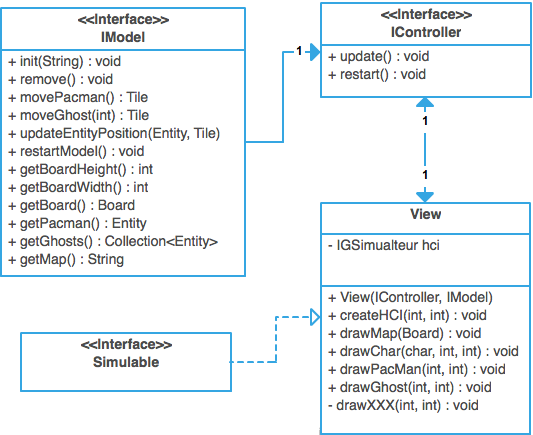
\includegraphics[scale=0.5]{MVC}}


\subsection{La gestion des personnages}

Les personnages sont la pièce maîtresse de l'application. Pour la simulation il y a deux types de personnages : Pacman et les fantomes.
Ci dessous, le diagramme de classes lié aux personnages : \\[0.5cm]
\centerline{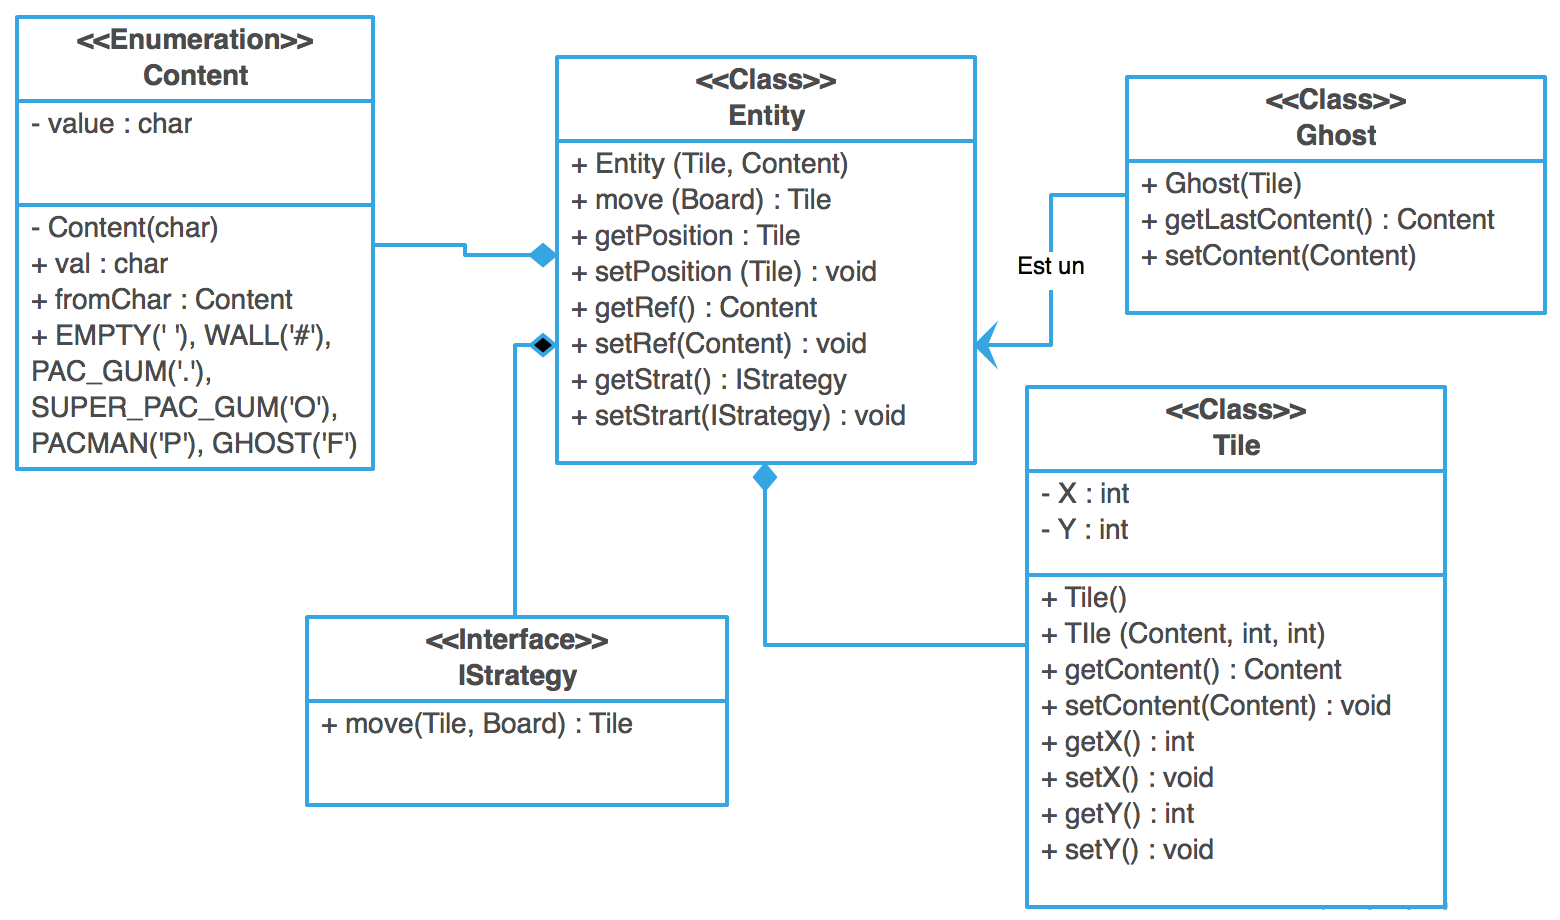
\includegraphics[scale=0.2]{Entity}}

Le premier choix était de savoir si Pacamn et les fantômes seraient des classes à part entière. La seule différence notable est le fait que Pacman mange tout ce qu'il trouve sur son chemin (excepté les fantomes) tandis que les fantomes doivent se déplacer sans altérer le contenu des cases qu'ils parcourent (excepté Pacman). C'est pourquoi la classe Ghost a un attribut lastContent afin de sauvegarder le contenu (cf Enum Content dans le diagramme) de la case sur laquelle le fantome se trouve.
Ceci permettra notamment de redessiner correctement la carte après passage d'un fantome. \\
D'autre part les points communs de tous les personnages sont le fait qu'ils se deplacent. Ce déplacement nécessite donc que chaque personnage possède une position, sa position courante. La classe Tile (cf partie Gestion de la carte) sert à stocker l'emplacement de nos personages. La méthode move() du personnage retourne la nouvelle position du personnage et délègue ce calcul à la stratégie (cf partie sur les Stragtégies) du personnage.



\subsection{Les stratégies de déplacement d'un personnage}

Notre projet inclut des stratégies car les personnages peuvent en effet se déplacer de différentes manières en fonction du contexte ou en fonction du choix de l'utilisateur. Comme le montre le diagramme ci après, chaque stratégie correspond à un type de déplacement (les algorithmes sont expliqués plus loin). \\[0.5cm]

\centerline{\includegraphics{}}

La méthode move() de chaque stratégie prend en paramètre un Board (cf Gestion des cartes) et une Tile représentant la position courante d'un personnage sur le jeu. La méthode retourne la nouvelle position du personnage.


\subsection{Gestion de la carte}

Le modele du MVC permet de stocker toutes les données de la simulation. Un carte est un tableau en deux dimensions de taille fixe qui contient des éléments de type Content. Ainsi au démarrage de l'application le modele est initialisé en parsant le fichier de carte sur lequel on veut jouer. Les données lues au moment du parsing sont stockées dans un objet de type Board dont voici la description : \\[0.5cm]
\centerline{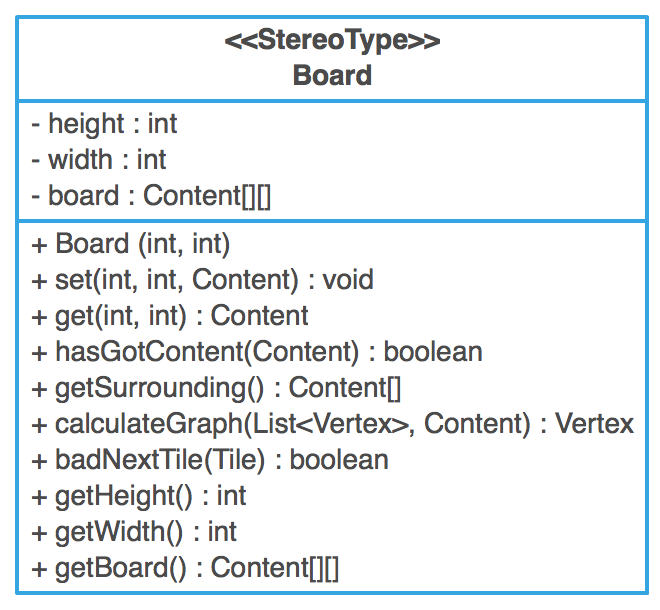
\includegraphics[scale=0.2]{Map}}

Le choix du tableau de taille fixe nous permet d'autre part de gérer les fichiers malformés, les dépassement ce tableau... En effet, c'est grâce à cette objet que nous pouvons tester les cartes "invalides" (les cartes où Pacman ne pourra jamais gagner car il est bloqué).

\subsubsection{vérification de la carte}

Lors du chargement d'une carte une vérification est effectuée afin de déterminer si toutes les pommes de la carte sont accessible par Pacman et si les Fantomes peuvent atteindre Pacman. Pour cela la classe BoardChecker contient une méthode qui va d'abord compter le nombre de cases qui ne sont pas un mur puis sélectionner la première case rencontrée remplissant ces conditions (à condition que la carte ne soit pas composée uniquement de murs). Ensuite l'algorithme visite les cases voisines récursivement jusqu'à avoir visité toutes les cases accessibles par la case d'origine. Le nombre de cases visité est enfin comparée au nombre de cases non-mur total et si ils sont différents, une exception est levée et le programme s'arrête, sinon le jeu peut démarrer.


Nous avons essayé au travers de cette application de mettre en place des mécanismes de Progammation Orientée Objet tels que les designs patterns (MVC, Strategy), l'héritage... D'autre part, nous avons tenté de découper le code afin que le travail en équipe soit facilité dans le sens où la compréhension de chaque fonction ou classe soit la plus claire et plus rapide pour chaque membre du groupe.

% Section 3 : conditions de victoire
\subsection{Les conditions de victoire}

A chaque tour de jeu le programme vérifie les conditions suivantes: \\
\begin{itemize}
	\item Il reste des pommes ou super pommes sur la carte;
	\item Pacman et un fantome sont sur la même case.
\end{itemize}

Si l'une des deux condition est remplie, une exception GameEndedInterrupt est lancée et le jeu s'arrête avec le résultat de la partie (Pacman a gagné ou les fantomes ont gagnés) affiché dans la console Java.

%Section 4 : Les algorithmes
\section{Les algorithmes}

%Sub 1 : Random
\subsection{Déplacements aléatoires}

L'algorithme de déplacement alétoire récupère tout d'abord pour chaque personnage sa position actuelle sur le tableau. Ensuite, il récupère les cases voisines (droite/gauche et haut/bas) puis en sélectionne une au hasard. Si la case sélectionnée est un mur il rétière la sélection sinon il retourne la case sélectionnée pour que le programme effectue le déplacement.

%Sub 2 : Plus court chemin
\subsection{Algorithme du plus court chemin}

%Subsub 1 : Choix de l'algorithme
\subsubsection{Choix de l'algorithme}

Pour le calcul du plus court chemin nous avons fait le choix d'appliquer l'algorithme de Dijkstra. C'est un algorithme simple, efficace et que nous avons vu cours de Recherche Operationnelle. Pour l'implémentation nous avons créé un package Djikstra comportant les classes suivantes:
\begin{itemize}
	\item Vertex: cette classe correspond au noeuds du graphe utilisé pour l'algorithme;
	\item Edge: cette classe correspond au arc entre 2 noeuds adjacents;
	\item Djikstra: cette classe permet de calculer le plus court chemin entre un source et un objectif.
\end{itemize}

%Diagramme UML
\centerline{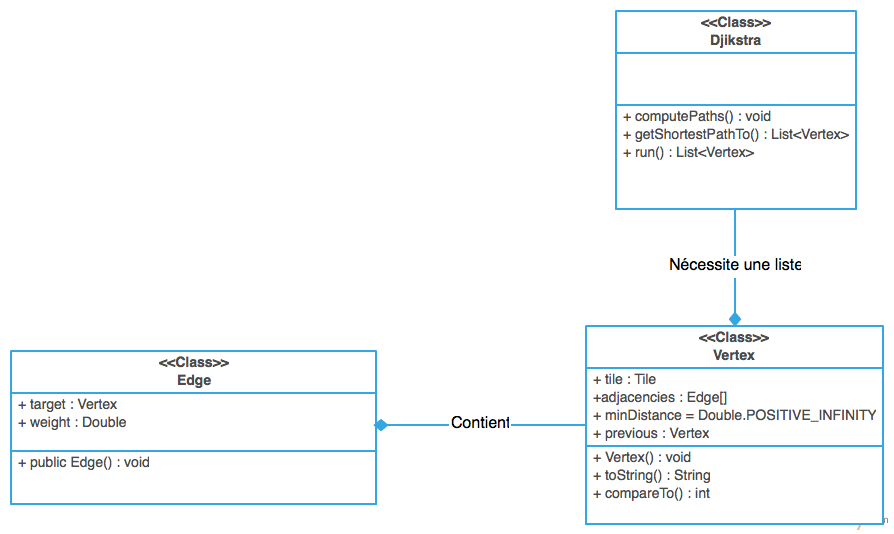
\includegraphics[scale=0.5]{Djikstra}}

Le calcul du plus court chemin se deroule en suivant les étapes qui suivent:
\begin{itemize}
	\item Créer une liste repertoriant tous les noeuds de la carte, c'est-à-dire créer une liste de Vertex;
	\item Pour chaque, noeuds déterminer qui sont ses voisins et le poids du passage du noeud A au noeud B (pas defaut 1). Cela correspond a un tableau de Edge;
	\item Lancer l'algorithme de Dijkstra avec la methode run() en précisant le point de depart et le point point d'arrivé dans les paramètres. 
	\item Le chemin retourné est une liste de Vertex correspondant au chemin à suivre.
\end{itemize}

%Subsub 2 : Tests et probl�mes rencontr�s
\subsubsection{Tests et problemes rencontres}
blabla

%Subsub 3 : Piste d'am�lioration
\subsubsection{Améliorations possibles}

Cette fonctionnalité n'est pas parfaite et plusieurs amélioration serait possible. Premièrement si Pacman et les Ghosts ont pour statégie le plus court chemin alors le résultat obtenu n'est pas celui souhaité. De plus, il est possible que Pacman se fasse manger par un Ghost. Quand un chemin est calculé Pacman va suivre se chemin, et l'évaluation de la viabilité de la case suivante n'est pas totalement fonctionnelle. Dans certains cas, la case suivante vers laquelle il va se diriger est aussi une case adjacente à un ghost. Et il arrive que Pacman et un Ghost se retrouvent au même endroit. Une méthode badNextTile() est présente pour évaluer cette viabilité mais son fonctionnement n'est pas opérationnel.\\
Le calcul de plus court chemin entre un point A et un point B fonctionne. Mais un ajout d'intelligence pour faire face à certaines situations pourrait être un axe d'amélioration.


%Sub 3 : minimax
\subsection{Minimax}

\end{document}

